\section{Experiments and Results}
\label{sec:experiments}

\textbf{Setup.} I2I 2025v1 slices from DeepLesion~\cite{yan2018deeplesion} ($512 \times 512$, $[0, 1]$) with
Poisson-simulated low-dose versions~[TODO cite]; training input $10^5$ photons; patient-level split of 899, 182 and 220
slices (115, 34, 31 patients). All eleven configurations (C0 is L1 only) train the same U-Net~\cite{ronneberger2015unet}
with AdamW ($10^{-4}$), batch 8, 30 epochs and mixed precision, keeping the checkpoint with the lowest validation L1.
Seeds 42, 123 and 456 vary the denoiser training only; $\lambda_\phi$ and the CT dose network are fixed. Code:
TODO(link).
% DISCUSS (pending supervisor reply): "checkpoint selection unaffected" is the writing plan's wording.
Validation L1 in eval mode spikes in some runs (up to 8 of 30 epochs), which leaves checkpoint selection unaffected;
one run (C8, seed 42) has no recorded code revision. Metrics: PSNR, SSIM, LPIPS (AlexNet)~\cite{zhang2018lpips},
DISTS, and the high-band noise power ratio $R_H$ at 0.25 to 0.5 cycles per pixel~\cite{samei2019tg233}, tested as
$\lvert 1 - R_H \rvert$. Family A compares C1 to C10 with C0, Family B C8 with C5, C10 with C9 and C6 with C5, on
PSNR, LPIPS and $\lvert 1 - R_H \rvert$ (Holm over 30 and 9 tests), with paired Wilcoxon tests over the 31 test
patients (seeds averaged per slice, slices per patient), effect size $r$ and seed spread; slice-level tests are in the
repository. Screen-versus-outcome Spearman correlations are exploratory: C5 and C8, C9 and C10, and C1 to C3 share
feature networks.

% Tue Oct 20: screen paragraph (Fig. 2), Table 1 paragraph, Fig. 3 and Fig. 4 paragraph (about 280 words).
TODO (Tue): results.

\begin{figure}[t]
  \centering
  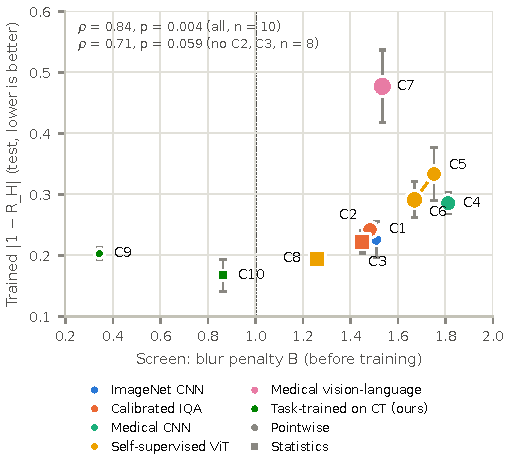
\includegraphics[width=0.75\linewidth]{figures/fig4_screen_vs_outcome}
  \caption{Blur penalty against trained texture error. The screen does not predict the trained result
    ($\rho = 0.84$, exploratory).}
  \label{fig:screen-outcome}
\end{figure}
